\documentclass[12pt]{article}
\setlength\parindent{0pt}
\usepackage{fullpage}
\usepackage{epsf}
\usepackage{amsmath}
\usepackage{graphicx}
\setlength{\parskip}{4mm}
\def\LL{\left\langle}   % left angle bracket
\def\RR{\right\rangle}  % right angle bracket
\def\LP{\left(}         % left parenthesis
\def\RP{\right)}        % right parenthesis
\def\LB{\left\{}        % left curly bracket
\def\RB{\right\}}       % right curly bracket
\def\PAR#1#2{ {{\partial #1}\over{\partial #2}} }
\def\PARTWO#1#2{ {{\partial^2 #1}\over{\partial #2}^2} }
\def\PARTWOMIX#1#2#3{ {{\partial^2 #1}\over{\partial #2 \partial #3}} }
\newcommand{\BE}{\begin{displaymath}}
\newcommand{\EE}{\end{displaymath}}
\newcommand{\BNE}{\begin{equation}}
\newcommand{\ENE}{\end{equation}}
\newcommand{\BEA}{\begin{eqnarray}}
\newcommand{\EEA}{\nonumber\end{eqnarray}}
\newcommand{\EL}{\nonumber\\}
\newcommand{\la}[1]{\label{#1}}
\newcommand{\ie}{{\em i.e.\ }}
\newcommand{\eg}{{\em e.\,g.\ }}
\newcommand{\cf}{cf.\ }
\newcommand{\etc}{etc.\ }
\newcommand{\Tr}{{\rm tr}}
\newcommand{\etal}{{\it et al.}}
\newcommand{\OL}[1]{\overline{#1}\ } % overline
\newcommand{\OLL}[1]{\overline{\overline{#1}}\ } % double overline
\newcommand{\OON}{\frac{1}{N}} % "one over N"
\newcommand{\OOX}[1]{\frac{1}{#1}} % "one over X"

\pagenumbering{gobble}

\begin{document}


\bigskip
\bigskip
\bigskip
\bigskip

\Large \centerline{\sc{Physics 211 Practice Exam 3}}
\normalsize

{\bf Question 1:}

A rope is wound around a spool with radius $R$ and mass $M$. A bucket of mass $m$ hangs from the spool, suspended over a well of depth $h$. The bucket is released from rest and falls down the well, spinning the spool as it does so.

\begin{enumerate}
  \item{In terms of the tension $T$ in the rope and the other given quantities, what is the angular acceleration of the spool?}
  \item{In terms of the tension $T$ in the rope and the other given quantities, what is the linear acceleration of the bucket?}
  \item{In terms of $R$, $M$, $m$, $h$, and $g$, how long does it take the bucket to hit the bottom of the well?}
  \item{Suppose I instead asked the question ``How fast will the bucket be traveling when it reaches the bottom?'' What other technique might you use that will let you answer this with a single equation? Write that equation down and solve it.}
\end{enumerate}

{\bf Question 2:}

A person tries to support a pipe of length 2 meters from one end horizontally. This pipe has a mass of 10 kg. If he puts one of his hands on one end of the pipe, and the other one 50 cm from the end, 
find the forces (magnitude and direction) he must exert with each hand to keep the pipe from falling.

{\bf Question 3:}

Consider the demo we did in class: a student of mass 75 kg stands on the center of a rotating stool holds two masses of 2 kg each with his arms outstretched. Model the student as a cylinder of radius 20 cm, and suppose his arms extend one meter from the center of 
his body. Someone spins him at $\omega=2$ rad/s. 

\begin{enumerate}
  \item{If he then brings his arms to his chest, so that the masses are only 10 cm from the vertical axis, what is his new angular velocity?}
  \item{Compute his kinetic energy before and after the motion. If there is a difference in energy, to what do you ascribe this? ({\it This problem is more vague than those that will be on your exam.})}
\end{enumerate}
\newpage
{\bf Question 4:}

For each of the following quantities, tell whether it can be positive, negative, or zero. There may be multiple answers: for instance, if I said ``the number of pencils in my pocket'', you would say ``positive or zero''.

\begin{enumerate}
  \item{Kinetic energy}
  \item{Gravitational potential energy}
  \item{The change in total kinetic energy in a partially inelastic collision}
  \item{The work done by a normal force}
  \item{The work done by static friction}
  \item{The work done by the tension force in a pendulum}
  \item{The torque exerted by the Earth's gravity on the Moon, with the pivot point at the Earth}
  \item{The work done by a baseball player on a baseball as he catches it}
  \item{The work done by an archer's hand on the arrow as she draws a bow}
  \item{The work done by the bowstring on the arrow as an archer draws a bow}
\end{enumerate}

{\bf Question 5:}

Problem 12.62, page 351, reproduced here:

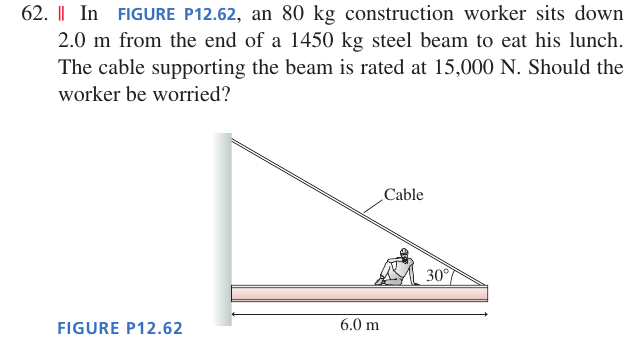
\includegraphics[width=0.5\textwidth]{torque1.png}
\newpage
{\bf Question 6:}

Problem 12.68, page 351, reproduced here:

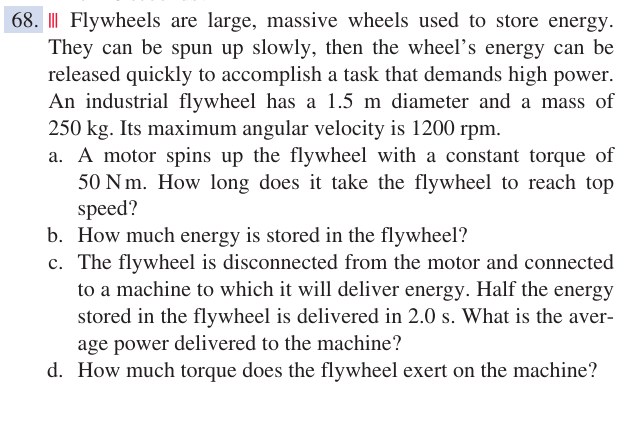
\includegraphics[width=0.5\textwidth]{kinematics1.png}

{\bf Question 7:}

  A person rolls a solid cylinder and a ball, each of radius $r=10$ cm and mass $m=2$ kg, toward a ramp at $v_0 = 3 \rm m/\rm s$. The ramp makes a $40^o$ degree angle with the horizontal.
    How far will each object travel up the ramp? What if the ball's radius is changed to 5 cm?

{\bf Question 8:}

A falconer training a falcon throws a lure of mass 200 g at an angle 45 degrees above the horizontal with an initial velocity of 15 m/s. One second after she throws it, her falcon catches it in mid-air. If the falcon has a mass of 400 g, and is diving straight
downward at 20 m/s when he catches it, how fast is the falcon traveling afterwards, and in what direction?



\end{document}



